\documentclass{beamer}
\usepackage{graphicx}
\usepackage[T1]{fontenc}

\title{Kanto: FPGA Audio Player and Visualizer}
\author{
  Kavita Jain-Cocks
  \and
  Zhehao Mao
  \and
  Amrita Mazumdar
  \and
  Darien Nurse
  \and
  Jonathan Yu}

\begin{document}
\begin{frame}
	\titlepage
\end{frame}

\begin{frame}{Project Overview}
	\begin{itemize}
		\item Objective: Design and implement an audio player with frequency visualization.
		\item Hardware: Handles audio output and frequency visualization
		\item Software: Handles user interaction and system initialization
	\end{itemize}
\end{frame}

\begin{frame}{High-Level Overview}
	\centering
	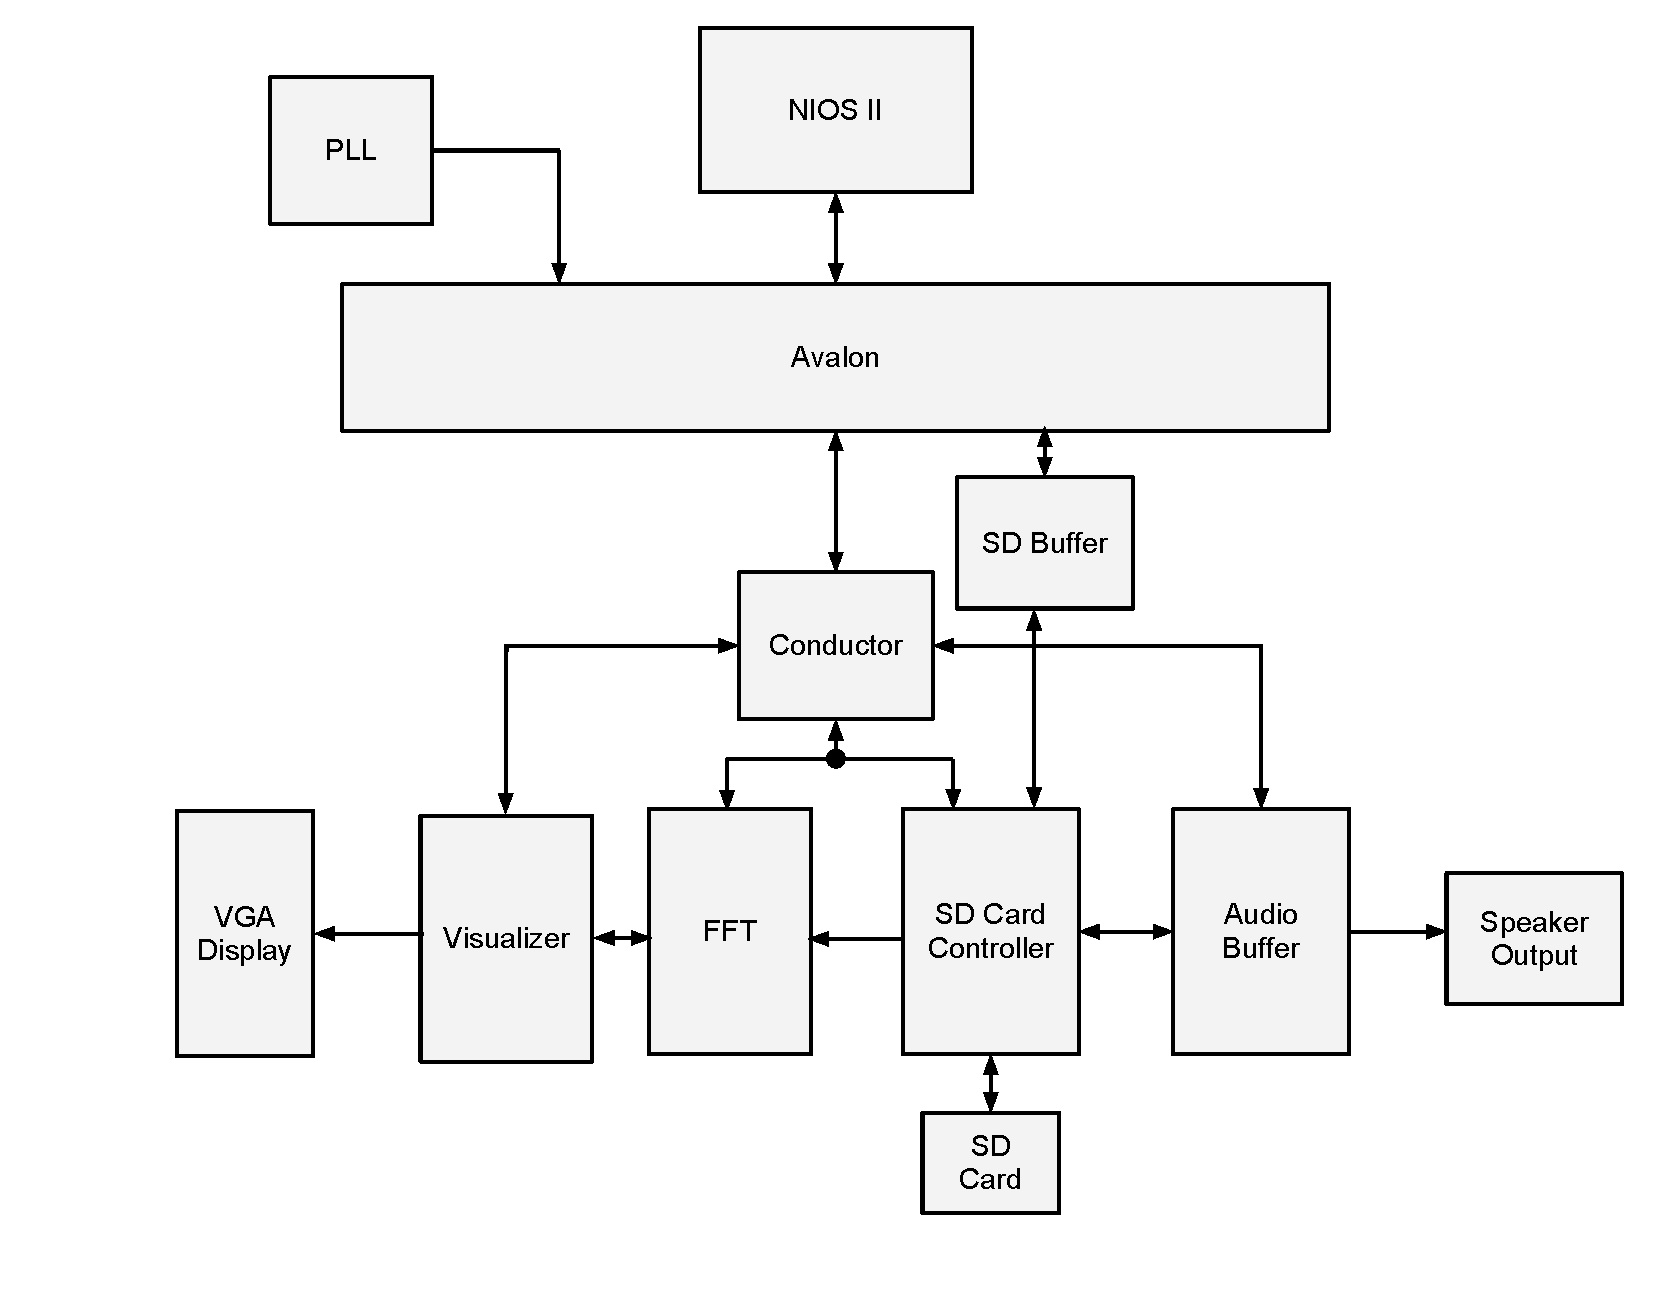
\includegraphics[width=4in]{top_level}
\end{frame}

\begin{frame}{SD Controller}
	\centering
	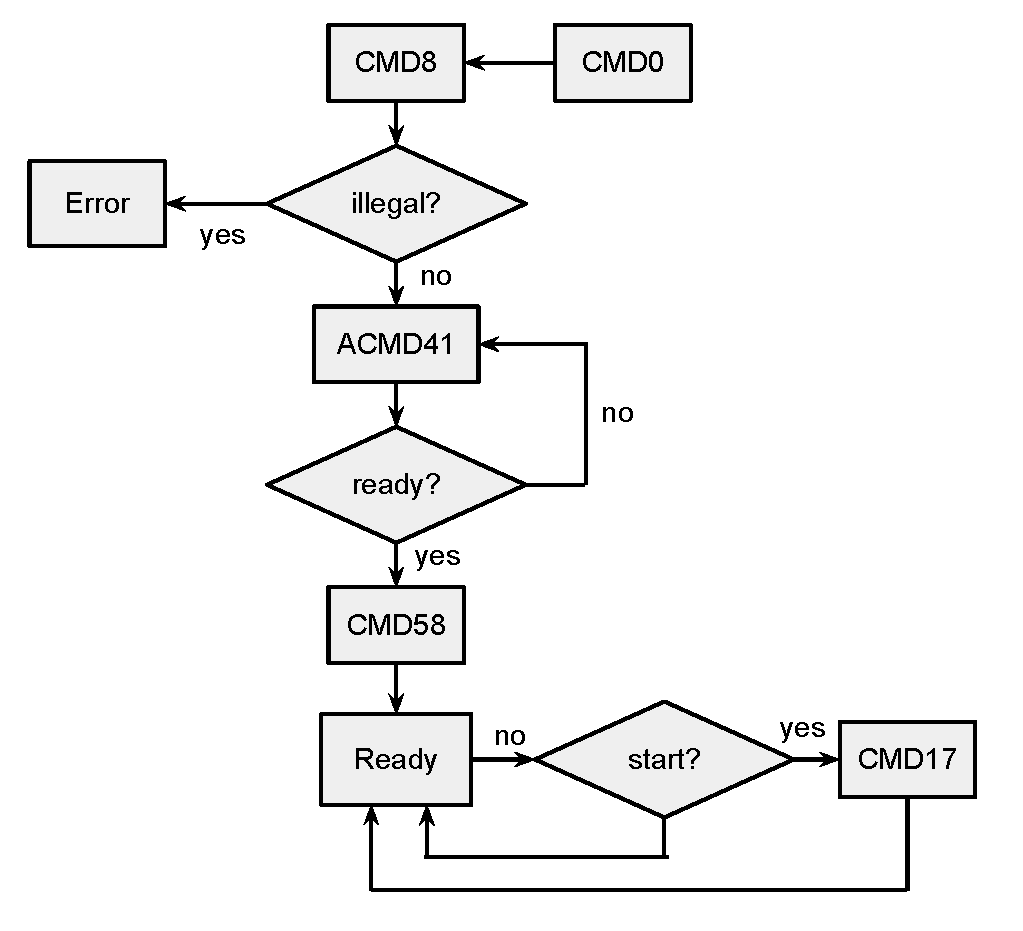
\includegraphics[height=3in]{sd-controller}
\end{frame}

\begin{frame}{Audio Buffer}
	\centering
	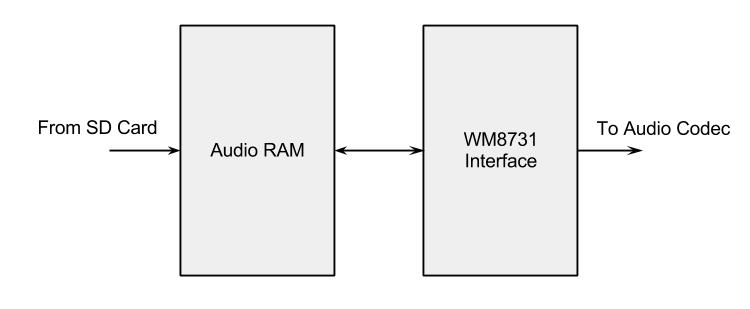
\includegraphics[width=4in]{audio-buffer}
\end{frame}

\begin{frame}{FFT Top-Level}
	\centering
	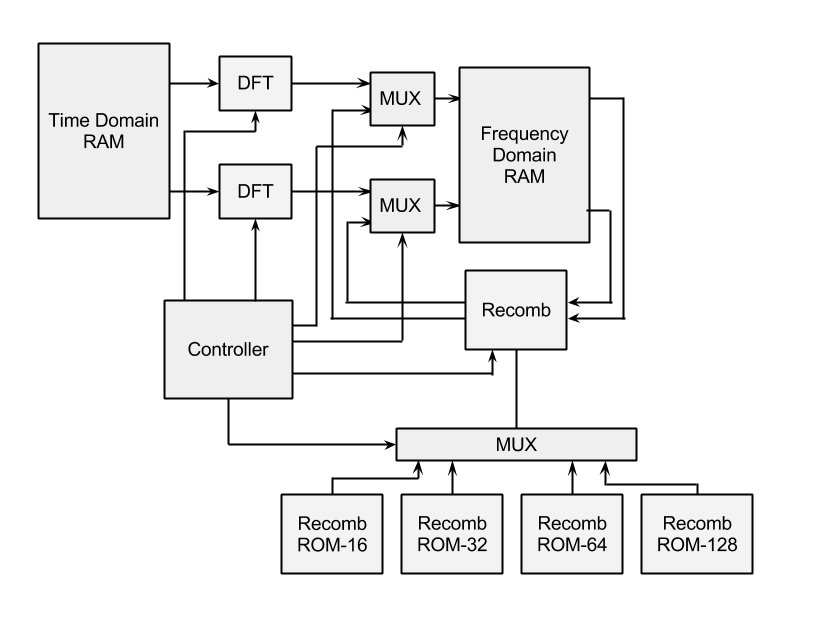
\includegraphics[width=4in]{fft-top}
\end{frame}

\begin{frame}{DFT Unit}
	\centering
	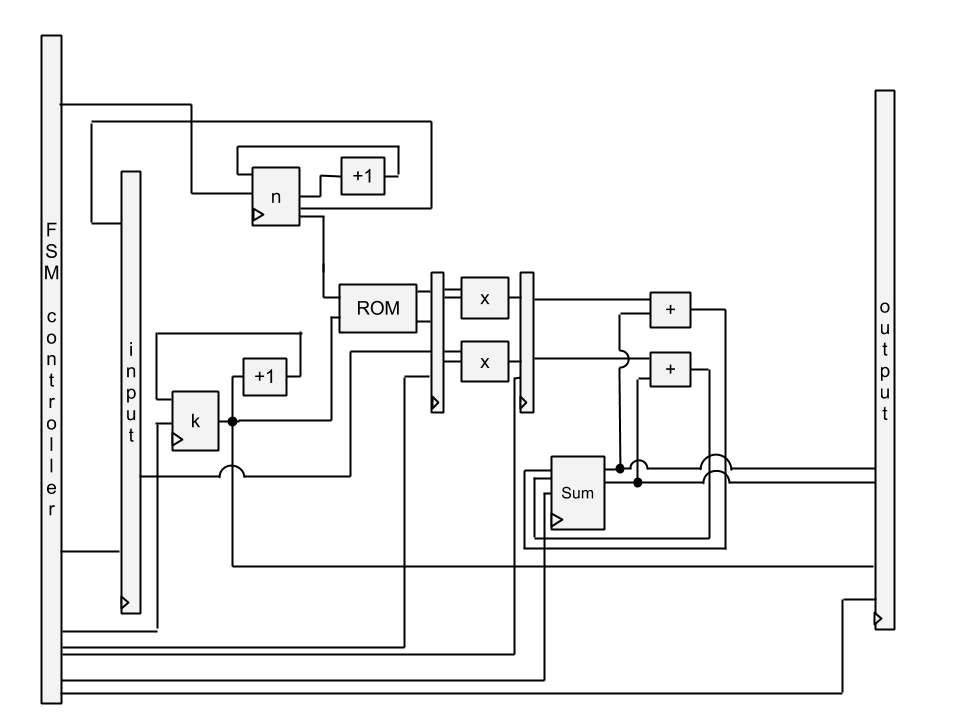
\includegraphics[width=4in]{dft-unit}
\end{frame}

\begin{frame}{Recombination Unit}
	\centering
	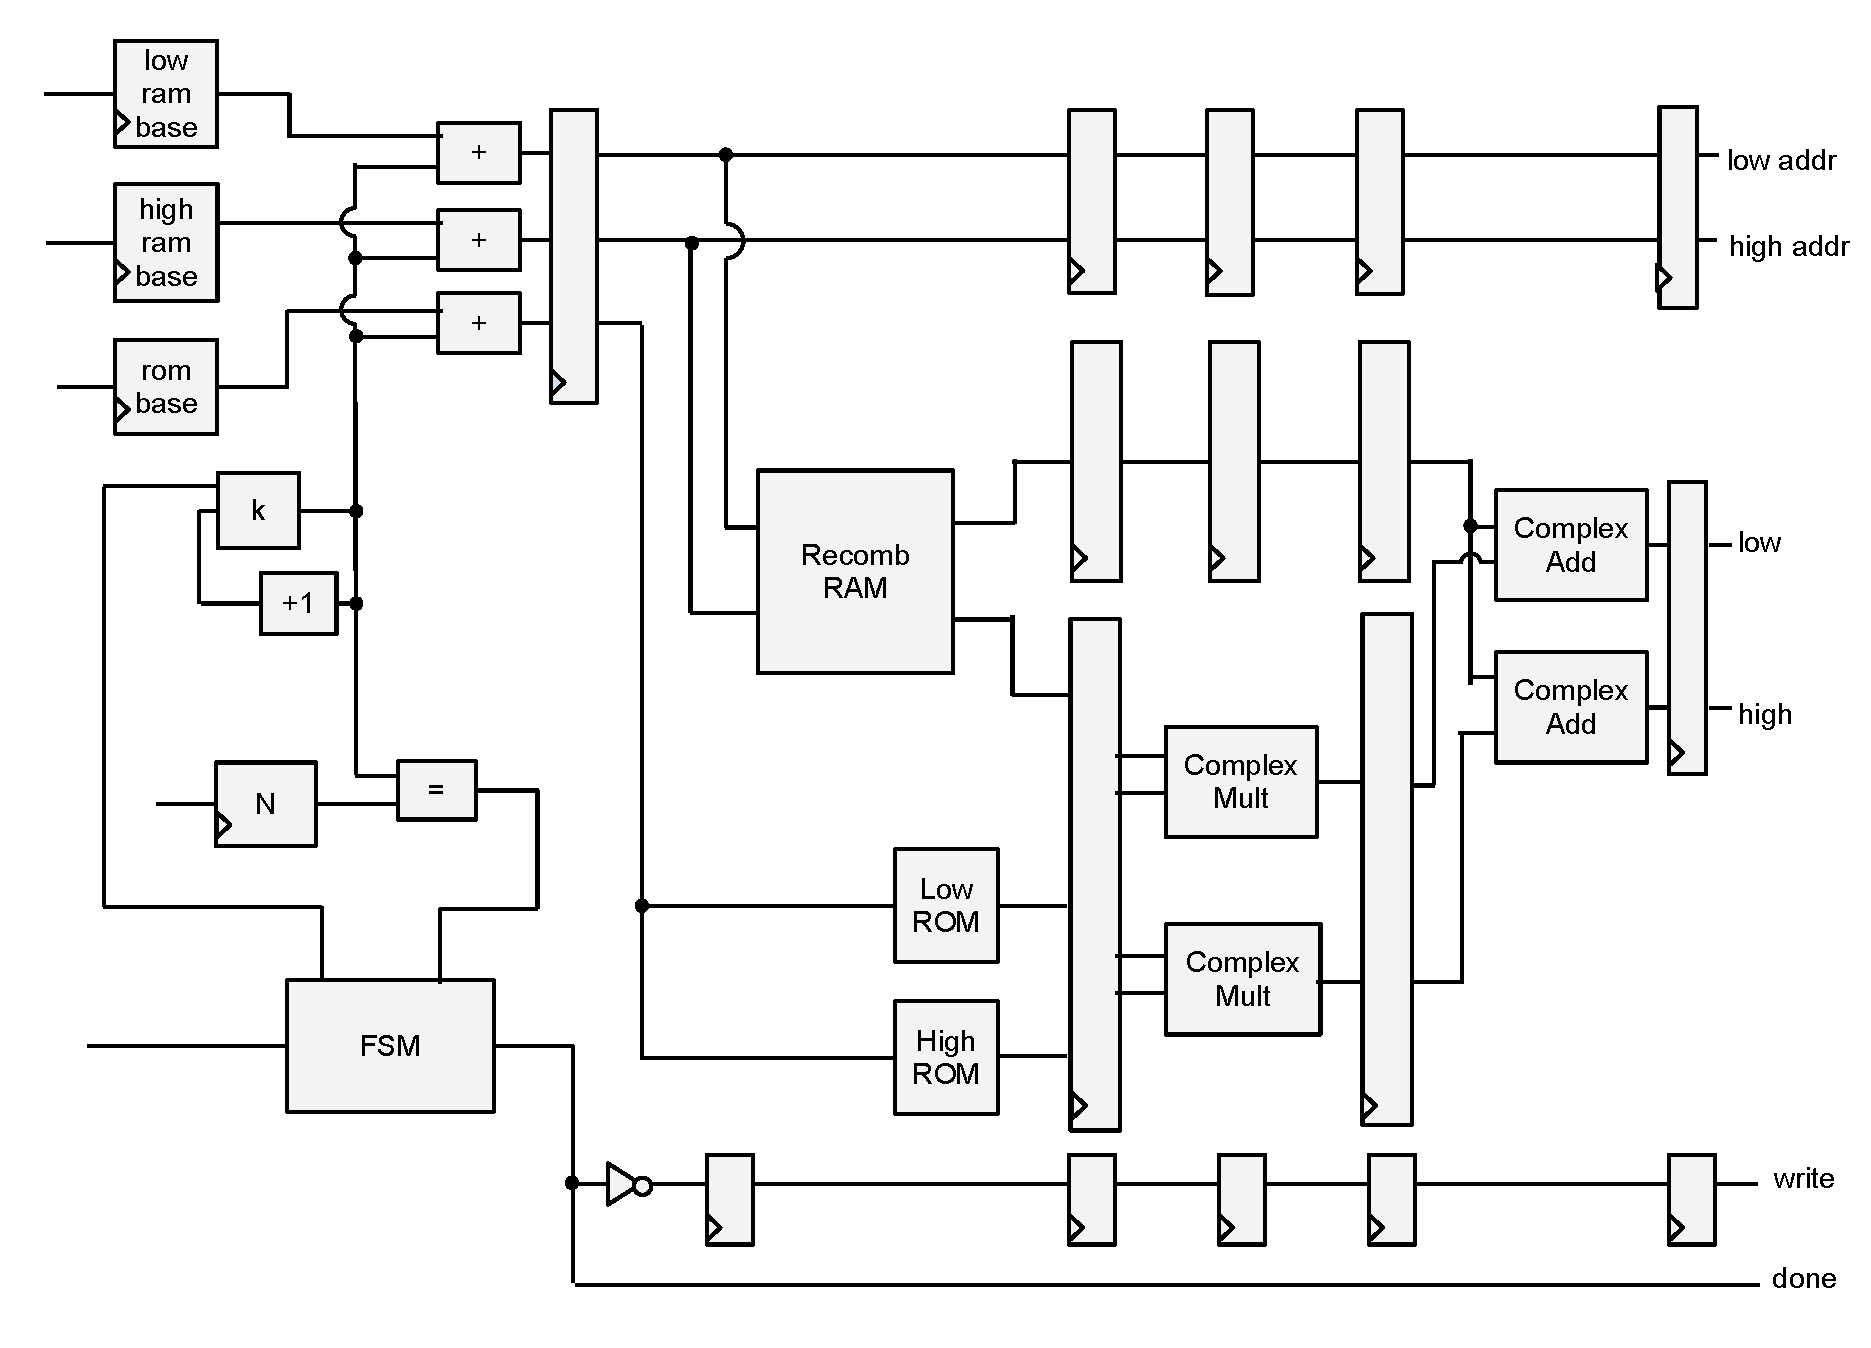
\includegraphics[width=4in]{recombinator}
\end{frame}

\begin{frame}{Complex Multiplier}
	\centering
	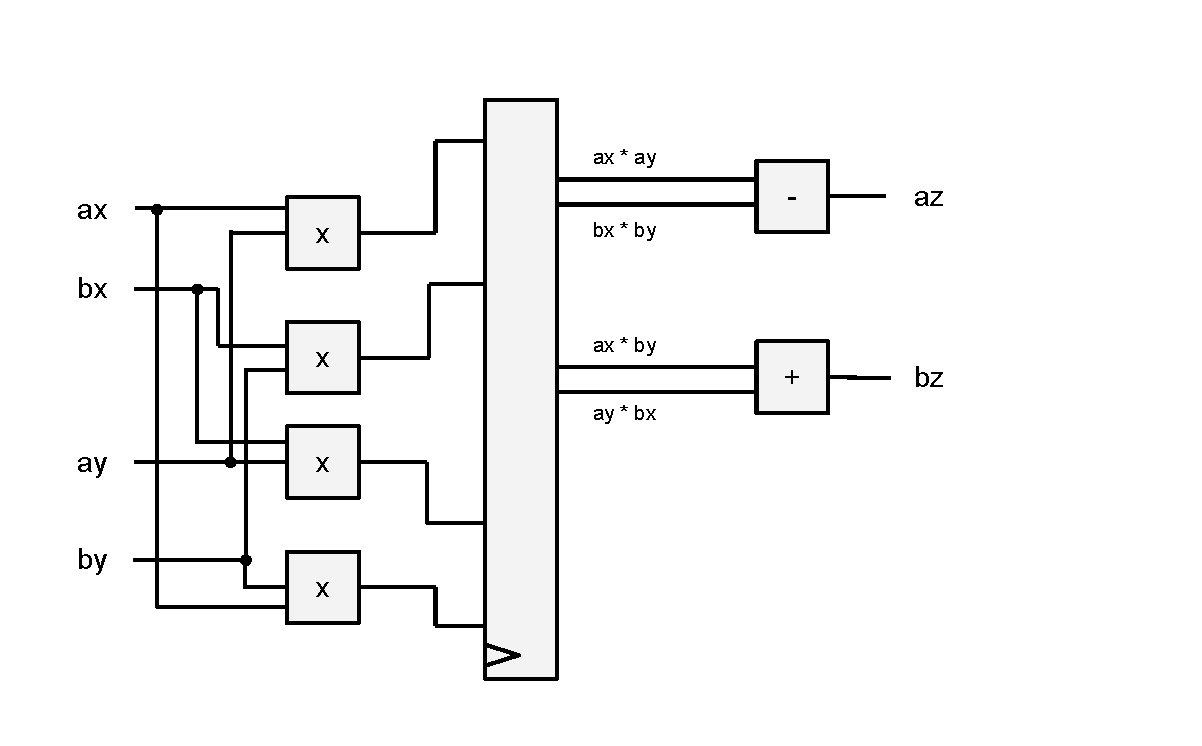
\includegraphics[width=4in]{complex-mult}
\end{frame}

\begin{frame}{Visualizer}
	\centering
	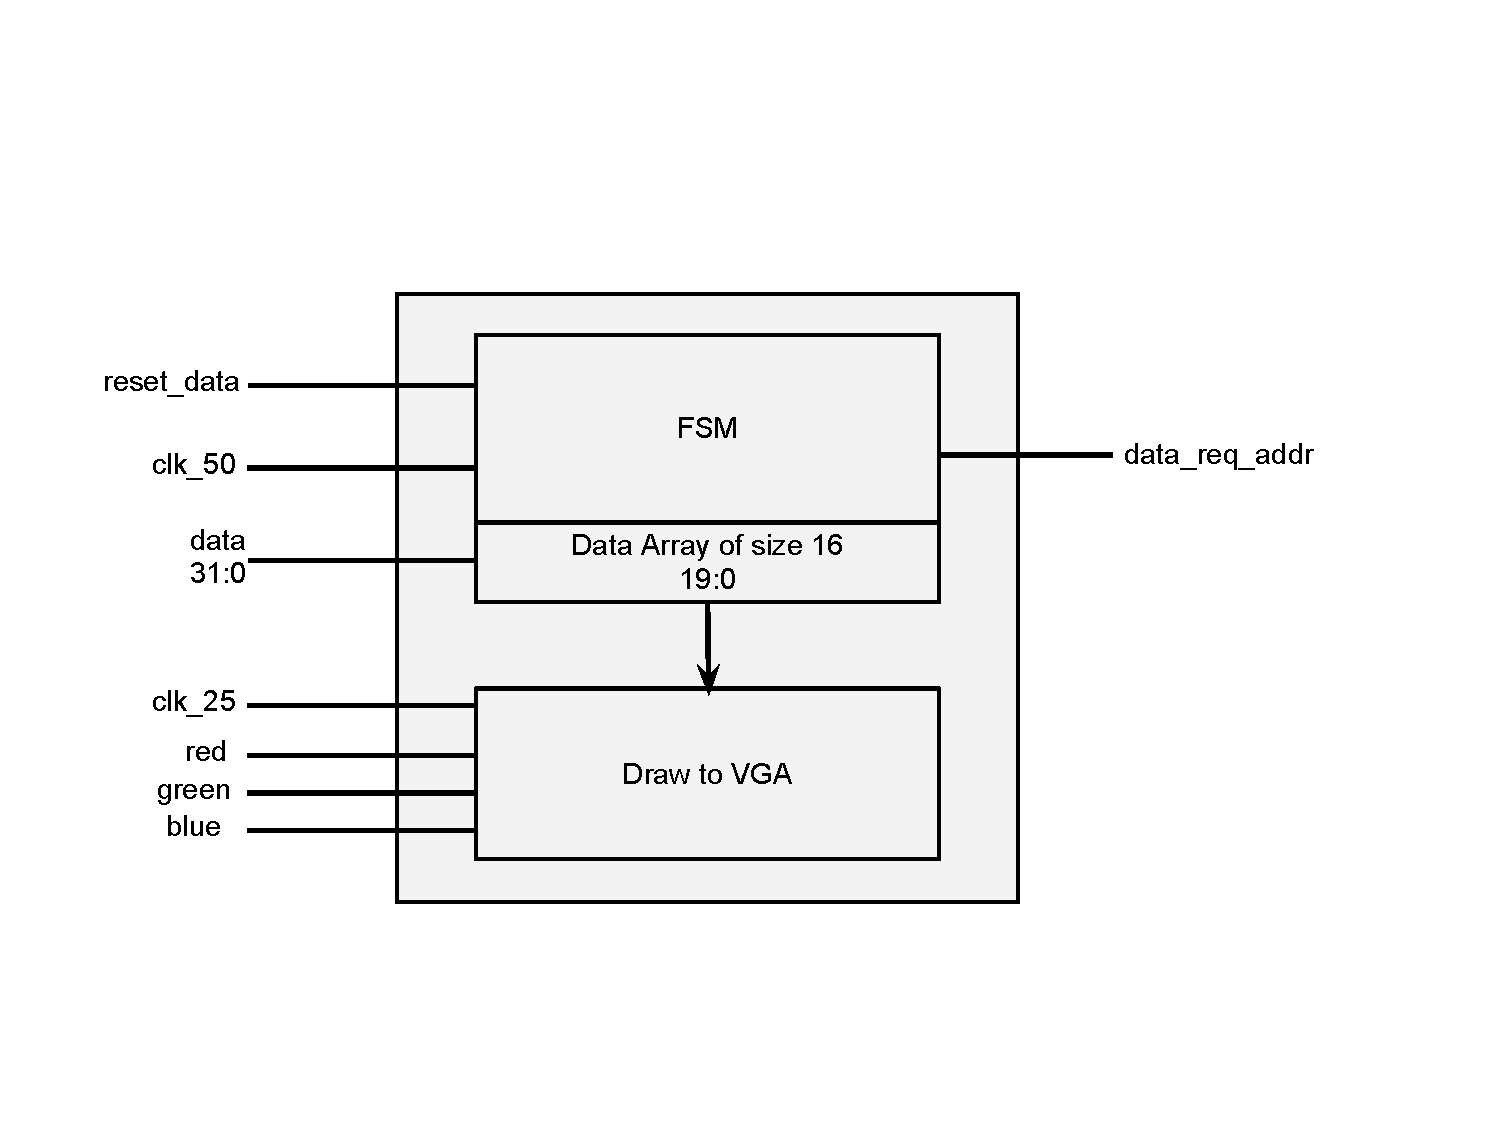
\includegraphics[width=4in]{viz_block_diagram}
\end{frame}

\begin{frame}{Conductor}
	\centering
    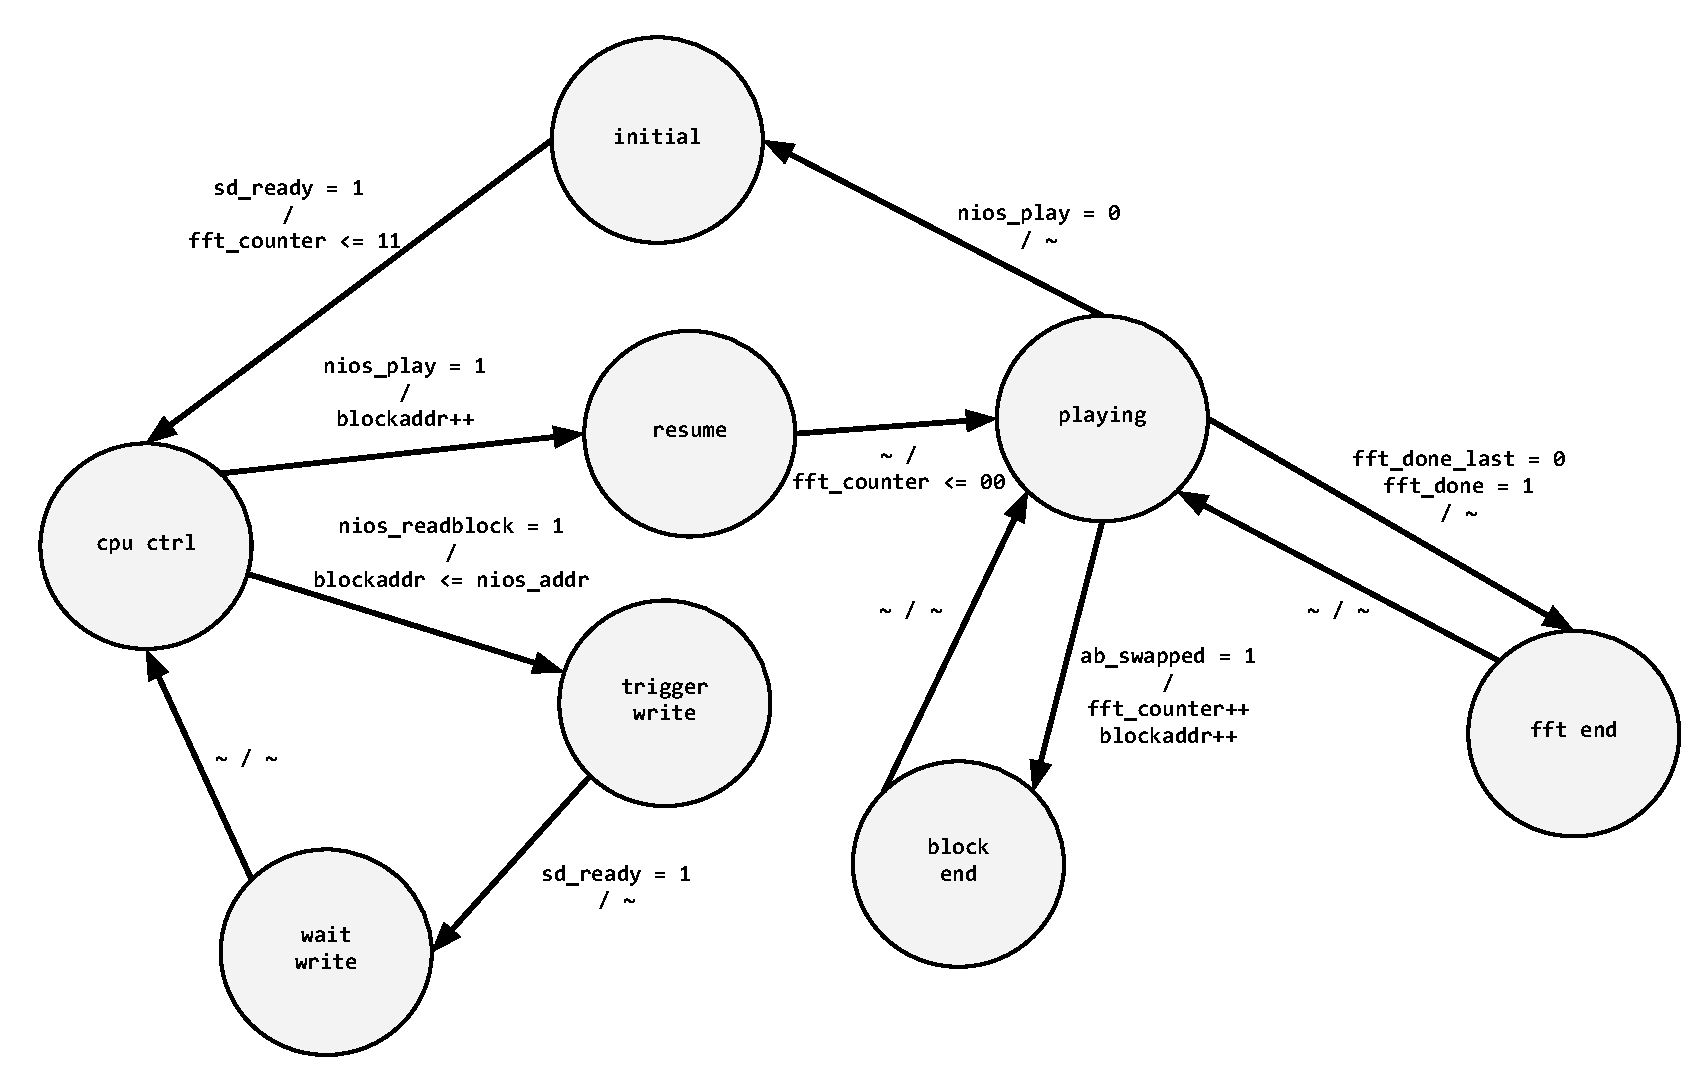
\includegraphics[width=4in]{conductor_state}
\end{frame}

\begin{frame}{Design Changes}
	\begin{itemize}
		\item Removal of SRAM
		\item Adding Software Control
		\item Display Changes
	\end{itemize}
\end{frame}

\begin{frame}{Lessons Learned}
	\begin{itemize}
		\item Clearly define milestones
		\item Communicate often and clearly with each other and the adviser
		\item Testbench everything
		\item Connect components early
		\item Implement modularized design
		\item Determine level of parallelism beforehand
	\end{itemize}
\end{frame}

\begin{frame}{The Hard Parts}
	\begin{itemize}
		\item Interfacing to external hardware (SD card, audio codec, visualizer) 
		\item Changing Levels of Parallelism 
		\item Timing Issues
		\item Reducing Hardware Usage
	\end{itemize}
\end{frame}

\end{document}
